    \item Let $\vec{N}$ be a $3$ by $3$ matrix with real number entries. The matrix $\vec{N}$ is such that $\vec{N}^{2}=0$. The eigenvalues of $\vec{N}$ are
    \hfill{\brak{\text{GATE IN 2018}}}
    \begin{enumerate}
        \begin{multicols}{4}
            \item $0,0,0$
            \item $0,0,1$
            \item $0,1,1$
            \item $1,1,1$
        \end{multicols}
    \end{enumerate}
    \item Consider the following system of linear equations
    \begin{align*}
    3x+2ky&=-2\\
    kx+6y&=2
    \end{align*}
    Here $x$ and $y$ are the unknowns and $k$ is a real constant. The value of $k$ for which there are infinite number of solutions is
    \hfill{\brak{\text{GATE IN 2018}}}
    \begin{enumerate}
        \begin{multicols}{4}
            \item $3$
            \item $1$
            \item $-3$
            \item $-6$
        \end{multicols}
    \end{enumerate}
    \item In the given circuit, the mesh currents $I_{1}$, $I_{2}$ and $I_{3}$ are
    \begin{figure}[H]
        \centering
        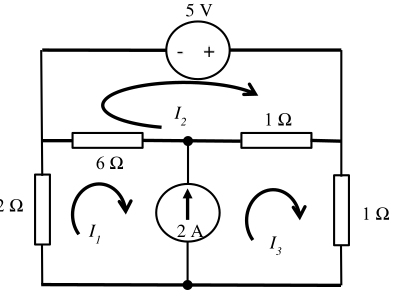
\includegraphics[width=0.7\columnwidth]{GATE/2018/IN/figs/q32.png}
        \caption{}
        \label{fig:q32}
    \end{figure}
    \hfill{\brak{\text{GATE IN 2018}}}
    \begin{enumerate}
        \begin{multicols}{2}
            \item $I_{1}=1$ A, $I_{2}=2$ A and $I_{3}=3$ A
            \item $I_{1}=2$ A, $I_{2}=3$ A and $I_{3}=4$ A
            \item $I_{1}=3$ A, $I_{2}=4$ A and $I_{3}=5$ A
            \item $I_{1}=4$ A, $I_{2}=5$ A and $I_{3}=6$ A
        \end{multicols}
    \end{enumerate}
    \item For the sequence $x[n] = \{1, -1, 1, -1\}$, with $n = 0,1,2,3$, the DFT is computed as $X\brak{k} = \sum_{n=0}^{3} x[n]e^{-j\frac{2\pi}{4}nk}$, for $k = 0,1,2,3$. The value of $k$ for which $X\brak{k}$ is not zero is
    \hfill{\brak{\text{GATE IN 2018}}}
    \begin{enumerate}
        \begin{multicols}{4}
            \item $0$
            \item $1$
            \item $2$
            \item $3$
        \end{multicols}
    \end{enumerate}
    
